% Capitulo 1

\chapter{Introducción} % Main chapter title

\label{Introduccion} % For referencing the chapter elsewhere, use \ref{Chapter1} 

\lhead{Capítulo 1 \emph{Introducción}} % This is for the header on each page - perhaps a shortened title

%----------------------------------------------------------------------------------------

En la actualidad, un dispositivo móvil está presente en los procesos de decisión en buena parte de lo que hacemos. Por ejemplo: es el aparato que nos despierta, y es el principal canal de comunicación en nuestra vida tanto profesional, como personal.

Es por ello que el presente proyecto describe el desarrollo de la aplicación Traveler Assistant System For Mexico City (TASMC), se basa en dos factores que han influido de forma decisiva en la experiencia viajera: el incremento en la transportación aérea de pasajeros; así como la creciente utilización de los dispositivos móviles, y con ellos, la facilidad de encontrar y comparar precios para elegir los más convenientes de acuerdo a las posibilidades de cada persona, y con ello, la opción de personalizar al máximo los viajes. La planeación es la mejor manera de ahorrar dinero y tiempo en un viaje. La incorporación de un elemento como el móvil conectado a internet, añade  nuevos fenómenos que enriquecen la experiencia viajera; un ejemplo de dichos fenómenos es el acceso a numerosos servicios de geolocalización.

El sector turístico es uno de los que se han visto obligados a adaptarse a los nuevos usos de los dispositivos móviles. Las nuevas tecnologías han proporcionado al cliente de las agencias de viajes, líneas aéreas, y servicios de hotelería, una gran autonomía \cite{appsVIajar} para organizar sus viajes. De acuerdo a la encuesta nacional de ingresos y gastos de los hogares “ENIGH 2012” y el modulo de disponibilidad y uso de tecnología de la información en los hogares “MODUTIH 2012” la conectividad es de un 60\% en los dispositivos móviles provocando un cambio sustancial en el proceso tradicional de gestión de un viaje aéreo \cite{endutih}.

El proyecto que se plantea será diseñado y desarrollado para dispositivos móviles en dos fases: como primera fase, localizar espacios o servicios en un área predeterminada, estos puntos se mostraran con etiquetas dentro del plano arquitectónico. Inicialmente para facilitar la gestión del módulo de la aplicación, el ámbito se limitará al AICM. Como segunda fase, hacer posible la planeación y organización integral de viajes aéreos, incluyendo información del vuelo, relación de vuelos y hoteles, itinerario de actividades planeadas, listado para control de equipaje y seguimiento de vuelos a través de mapas.


%----------------------------------------------------------------------------------------
\section{Problemática}

Los viajeros tienen ciertas necesidades desde el momento que deciden viajar por el transporte aéreo, incluso deben considerar una serie de problemas que se les pueden presentar como se muestra a continuación:

\textbf{Necesidades:}

\begin{itemize}
	\item Conocer el precio y horario de los vuelos que los llevan a su destino.
	\item Buscar un hotel de su conveniencia para hospedarse.
	\item Hacer un itinerario de viaje.
\end{itemize}

\textbf{Problemas:}

\begin{itemize}
	\item Olvidar papeles importantes, como el pasaporte.
	\item Olvidar empacar algún objeto que les sea necesario.
	\item Llegar a destiempo a la cita en el aeropuerto debido a la falta de conocimiento de la ruta.
	\item No ubicarse correctamente dentro del aeropuerto.
\end{itemize}

Hoy en día los viajeros buscan la información para cubrir estas necesidades utilizando la Internet,  generalmente lo hacen visitando diferentes páginas Web para encontrar la opción que mejor se ajuste a sus necesidades. Por otro lado, los problemas que se muestran no siempre son considerados y llevan a consecuencias no muy agradables como el perder un vuelo.
\section{Solución Propuesta}

Tomando en cuenta las problematicas mensionadas, se plantea desarrollar una solución que permita al viajero aéreo de la Ciudad de México organizar de manera adecuada su viaje, ofreciendo así una herramienta útil para el ámbito de turismo en México.

La herramienta a desarrollar tendrá la arquitectura que se muestra en la Figura \ref{fig:Arquitectura}. 

\begin{figure}[htbp]
	\centering
		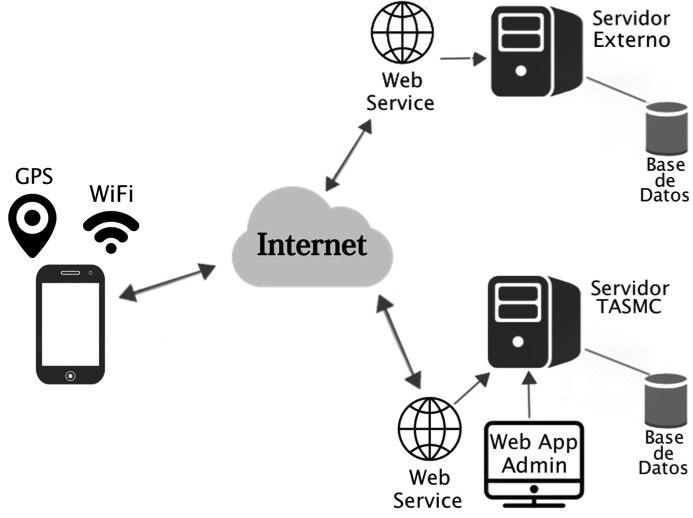
\includegraphics{Figuras/arquitectura.png}
		\rule{35em}{0.5pt}
	\caption[Diagrama de Arquitectura de TASMC]{Diagrama de Arquitectura de TASMC.}
	\label{fig:Arquitectura}
\end{figure}

A continuación se describe cada uno de los componentes que se muestran en la Figura \ref{fig:Arquitectura}:

\begin{itemize}
	\item \textbf{Dispositivo Móvil: }Cuenta con diferentes tecnologías que serán aprovechadas para el desarrollo de la aplicación, por lo tanto, la aplicación móvil será instalada en este dispositivo. Se conectará a la Internet para tener comunicación con el Web Service externo y con el que se desarrollará para este sistema.
	\item \textbf{Web Services: }Se visualizan dos en la Figura \ref{fig:Arquitectura}, uno es el externo que nos brindará la información correspondiente a hoteles y vuelos, y el otro que se desarrollará para brindar la información de los usuarios que utilizan la aplicación. 
	\item \textbf{Servidores: }Observamos dos en la Figura \ref{fig:Arquitectura} que son donde se alojan los Web Services y las Bases de Datos correspondientes, en el servidor TASMC también habrá aplicación Web.
	\item \textbf{Bases de Datos: }En este módulo encontramos los datos que se proveerán a la aplicación móvil y la aplicación Web.
	\item \textbf{Aplicación Web: }Es una aplicación que servirá para administrar a los usuarios, lugares y objetos de equipaje de la aplicación móvil.
\end{itemize}
\section{Alcances y Limitaciones}

El trabajo terminal tiene como alcance implementar una aplicación móvil que sea capaz de ubicar al usuario en el AICM, ayudando al mismo a encontrar la terminal y la sala en donde será su salida. También podrá localizar sitios de interés como alimentos y bebidas, compras, comunicaciones, servicios financieros,  servicios médicos, transportación terrestre y servicios turísticos.

El proyecto puede tener mayor alcance, ya que se podría extender en un futuro con otras funciones como información detallada de los sitios de interés buscados por el usuario, ofertas y promociones de los locales disponibles, consultas de catálogos, trazado de rutas desde el origen del usuario hasta su destino, etc.

Las limitaciones que presenta el proyecto tienen que ver con la información que se pueda obtener, ya que puede no existir un servicio que nos brinde el acceso a la base de datos de las aerolíneas y hoteles. 

Otra de las limitaciones es la localización en interiores ya que sigue siendo objeto de un intenso estudio e investigación para brindar una mejor exactitud cuando se utiliza alguna tecnología con este fin.


\section{Objetivo General}

Diseñar un sistema integral de gestión para las actividades de los viajeros del AICM, al brindarles la información necesaria en su dispositivo móvil para hacer posible la organización integral de viajes turísticos o de negocios en México.
\section{Objetivos Específicos}

\begin{itemize}
	\item	Configurar el viaje dependiendo de gustos y posibilidades económicas del viajero.
	\item	Sugerir los vuelos disponibles.
	\item 	Sugerir hoteles disponibles. 
	\item	Sugerir diferentes objetos que debe portar el viajero dependiendo del tipo de viaje.
	\item	Proporcionar las herramientas que permitan al usuario generar un itinerario de viaje.
	\item	Sugerir la mejor ruta para llegar al aeropuerto.
	\item	Ubicar al viajero dentro del AICM.
	\item	Visualizar un panel con información del número de vuelo, estado del vuelo,  ciudades de origen y destino, hora de salida y llegada, fecha, terminal y puerta.
\end{itemize}
\section{Justificación}

TASMC te va a proporcionar listados de hoteles, vuelos y objetos que debes considerar en tu equipaje y facilidades para generar un itinerario, hasta este punto es prácticamente lo mismo que te ofrecen otras aplicaciones. Sin embargo, existen dos novedades que nos diferencian de dichas aplicaciones:

\begin{enumerate}
	\item La ruta más conveniente para llegar al aeropuerto que se sugerirá dependiendo la distancia del  trayecto utilizando un servicio externo de geolocalización, esto se puede obtener con otras aplicaciones dedicadas específicamente a rutas, nosotros lo brindamos en una misma aplicación dedicada a la gestión integral del viaje.
	\item El punto más novedoso de nuestro sistema es la "Localización en Interiores", esta rama de la localización aun no es tan utilizada por diferentes razones, una de ellas es que el GPS carece de un funcionamiento tan eficaz en interiores comparándolo con el desempeño en exteriores. Nuestro sistema será el primero que implemente la localización en interiores para el AICM.  
\end{enumerate}

Nuestro proyecto beneficiará a todos los viajeros aéreos del AICM, independientemente del tipo de viaje. Por ejemplo, un viajero que no visita constantemente el aeropuerto le será de mucha utilidad la localización en interiores ya que le facilitará encontrar su sala de abordaje de una manera eficaz. Por otro lado, una persona que visita constantemente el AICM puede ubicarse con facilidad pero de ninguna manera puede perder su vuelo, lo cual se evitará utilizando nuestra sugerencia de rutas al aeropuerto. Finalmente, lo que se quiere es que el usuario de nuestro sistema tenga una mejor planeación, organización y control de su viaje, además de un ahorro de tiempo, combustibles y dinero, lo que se logrará con la información que el sistema proporcionará a través del móvil.
 
Finalmente, con el desarrollo de este trabajo terminal se busca aprovechar y hacer frente a las siguientes observaciones:

\begin{itemize}
	\item El turismo en México es una actividad fundamental en el desarrollo económico del país.
	\item El turista se enfrenta a un problema que puede dificultar su viaje al no tener bien organizado el mismo.
\end{itemize}

El sistema estará orientado a dispositivos móviles debido al constante crecimiento en el número de usuarios de este tipo de dispositivos y al acelerado avance tecnológico en los sistemas móviles, en particular, el sistema estará disponible para dispositivos móviles con el sistema operativo Android, esto debido a que actualmente es el sistema operativo líder en el mercado (ver Figura \ref{fig:moviles})\cite{moviles} y ofrece una mayor flexibilidad para el desarrollo de aplicaciones en comparación con sus principales competidores.

\begin{figure}[htbp]
	\centering
		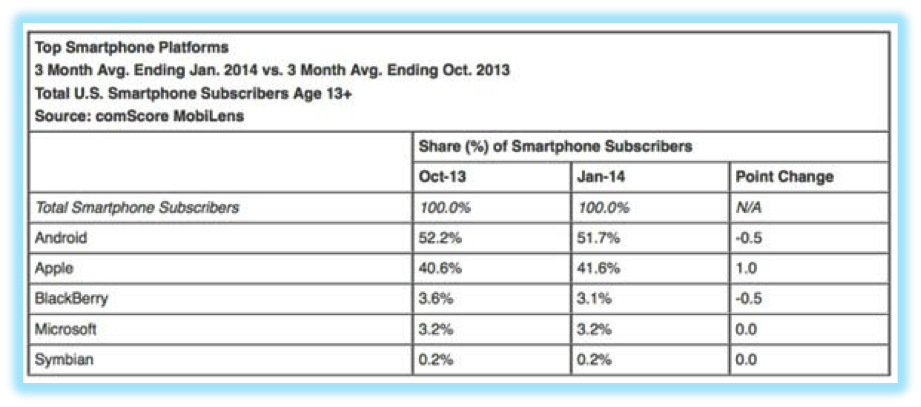
\includegraphics[width=1\textwidth]{Figuras/moviles.png}
		\rule{35em}{0.5pt}
	\caption[Mercado de los S.O. Móviles]{Presencia Actual en el Mercado de los S.O. Móviles}
	\label{fig:moviles}
\end{figure}